\documentclass[10pt,a4paper]{amsart}
\usepackage[margin=19mm]{geometry}
\usepackage{amsmath,amssymb,mathtools}
\usepackage[scr=rsfs,cal=euler]{mathalfa}
\usepackage{xfrac}
\usepackage[unicode,hidelinks,bookmarks=false]{hyperref}
\newcommand{\ie}{i.e.\ }
\newcommand{\cf}{cf.\ }
\newcommand{\resp}{respectively\ }
\newcommand{\Subsection}{\subsection}
\providecommand{\nobreakdash}{\nobreak\hbox{-}}
\setlength{\emergencystretch}{2em}
\multlinegap0pt
\usepackage{amsthm}
\usepackage{tikz}
\usepackage{tikz-cd}
\usepackage{pgfplots}
\usepackage{bbm}
\usepackage{enumitem}
% concatenated from uniqueness_draft_alt_inftro.tex
%\documentclass[11pt,letterpaper]{amsart}
%\usepackage{fullpage}

\usetikzlibrary{positioning}
\usetikzlibrary{calc, matrix, patterns}
\pgfplotsset{compat=1.10}
\usepgfplotslibrary{fillbetween}
\tikzset{fill between/on layer=main}
\usetikzlibrary{mindmap}

\DeclareFontFamily{U}{mathx}{}
\DeclareFontShape{U}{mathx}{m}{n}{<-> mathx10}{}
\DeclareSymbolFont{mathx}{U}{mathx}{m}{n}
\DeclareMathAccent{\widehat}{0}{mathx}{"70}
\DeclareMathAccent{\widecheck}{0}{mathx}{"71}


%%% Commenting macros.
\def\final{0}  % set this to 1 to get a comment-free version
\def\iflong{\iffalse}
\ifnum\final=0  %namely if we allow comments in the output
\providecommand{\kristof}[1]{{\color{red}[{\textbf{Kristóf:} \bf #1}]\marginpar{\color{red}*}}}
\providecommand{\marci}[1]{{\color{blue}[{\textbf{Marci:} \bf #1}]\marginpar{\color{blue}*}}}
\providecommand{\llaci}[1]{{\color{orange}[{\textbf{LLaci:} \bf #1}]\marginpar{\color{orange}*}}}
\providecommand{\tlaci}[1]{{\color{purple}[{\textbf{TLaci:} \bf #1}]\marginpar{\color{purple}*}}}
\providecommand{\greg}[1]{{\color{violet}[{\textbf{Greg:} \bf #1}]\marginpar{\color{violet}*}}}


\else % in this case [final=1] we don't want any comments to show
\providecommand{\kristof}[1]{}
\providecommand{\marci}[1]{}
\providecommand{\llaci}[1]{}
\providecommand{\tlaci}[1]{}
\providecommand{\greg}[1]{}
\fi

%%% Theorems, lemmas, claims, blah blah.
\theoremstyle{plain}
\newtheorem{thm}{Theorem}[section]
\newtheorem{lem}[thm]{Lemma}
\newtheorem{cor}[thm]{Corollary}
\newtheorem{cl}[thm]{Claim}
\newtheorem{obs}[thm]{Observation}
\newtheorem{prop}[thm]{Proposition}
\newtheorem{conj}{Conjecture}
\newtheorem{qu}[thm]{Question}
\newtheorem{prob}[thm]{Problem}

\theoremstyle{definition}
\newtheorem{defn}[thm]{Definition}
\newtheorem{note}[thm]{Notes}
\newtheorem{ex}[thm]{Example}
\newtheorem{assum}[thm]{Assumption}
\newtheorem{rem}[thm]{Remark}

%%% New definitions -- reals, epsilons, blah blah.
\providecommand{\R}{\mathbb{R}}
\providecommand{\Z}{\mathbb{Z}}
\providecommand{\N}{\mathbb{N}}
\providecommand{\Cay}{\mathrm{Cay}}
\providecommand{\Zpl}{\mathbb{Z}_{>0}}
\providecommand{\Znneg}{\mathbb{Z}_{\ge0}}
\providecommand{\overro}{\overline{\rho}}
\providecommand*\diff{\mathop{}\!\mathrm{d}}

\providecommand{\bF}{\mathbb{F}}
\providecommand{\bE}{\mathbb{E}}

\providecommand{\bK}{\mathbb{K}}
\providecommand{\bP}{\mathbf{P}}
\providecommand{\bR}{\mathbb{R}}
\providecommand{\cA}{\mathcal{A}}
\providecommand{\cB}{\mathcal{B}}
\providecommand{\cG}{\mathcal{G}}
\providecommand{\cS}{\mathcal{S}}
\providecommand{\cC}{\mathcal{C}}
\providecommand{\cV}{\mathcal{V}}
\providecommand{\cQ}{\mathcal{Q}}
\providecommand{\cE}{\mathcal{E}}
\providecommand{\cM}{\mathcal{M}}
\providecommand{\cN}{\mathcal{N}}
\providecommand{\cU}{\mathcal{U}}
\providecommand{\cF}{\mathcal{F}}
\providecommand{\cH}{\mathcal{H}}
\providecommand{\cK}{\mathcal{K}}
\providecommand{\mP}{\mathscr P}
\providecommand{\mC}{\mathscr C}


\providecommand{\cI}{\mathcal{I}}
\providecommand{\cJ}{\mathcal{J}}
\providecommand{\cO}{\mathcal{O}}
\providecommand{\cP}{\mathcal{P}}
\providecommand{\cT}{\mathcal{T}}
\providecommand{\cX}{\mathcal{X}}
\providecommand{\cY}{\mathcal{Y}}
\providecommand{\cZ}{\mathcal{Z}}
\providecommand{\cR}{\mathcal{R}}

\providecommand{\mm}{\text{mm}}
\providecommand{\mmp}{\mm^+}
\providecommand{\bmm}{\text{bmm}}
\providecommand{\bmmp}{\bmm^+}

\providecommand{\fg}{\varphi}
\providecommand{\eps}{\varepsilon}
\providecommand{\Haus}{{\text{\rm Haus}}}
\def\one{{\mathbbm1}}
\def\rk{\text{\rm rk}}
\tikzset{
		big dot/.style={
			circle, inner sep=0pt, 
			minimum size=1mm, fill=black
		}
	}
%%% Here comes the paper.


\title[Whitney 2-isomorphism theorem for graphings]{Whitney's 2-isomorphism theorem for graphings: measurable subtrees on the edges of a weakly 2-connected graphing (Lemma 3.5)}
\author[M. Borbényi, G. Terlov, L. M. Tóth]{Márton Borbényi, Grigory Terlov, László Márton Tóth}
\date{Source: arXiv:2605.16152v2 (CC BY 4.0)}
\begin{document}
\maketitle
\vspace{1em}
\noindent\textit{Source and licence.} Whitney's 2-isomorphism theorem for graphings. Version arXiv:2605.16152v2 (CC BY 4.0), distributed under the Creative Commons Attribution 4.0 International licence, http://creativecommons.org/licenses/by/4.0/, as recorded in the arXiv OAI licence metadata for this exact version and shown on the abstract page https://arxiv.org/abs/2605.16152v2. This item is an editorial re-presentation of the paper's measurable-subtree lemma together with the paper's own proof of it and the two source-local lemmas the statement and proof use. A full rights notice is delivered at licenses/arxiv-2605.16152-CC-BY-4.0.txt.
\noindent\textit{Editorial scope.} Counted unit: the paper's measurable construction of finite subtrees on the edges of a weakly 2-connected graphing, printed as Lemma 3.5 (source0.tex lines 1185--1193), delivered together with the paper's complete original proof of it (source0.tex lines 1195--1279) as the single primary proof body. No mathematics is written, repaired or re-derived: statement and proof are the paper's own text line for line, in the paper's own notation ($\cG$, $\cE$, $\cH$, $\cQ$, $C_{\cH}(e)$, $B_1^{\cQ}$, $T_e$). Required context retained uncounted, because the counted proof is the paper's own assembly over it: the two lemmas the statement and proof invoke, each with its own proof, namely the bipartite triangle lemma (source0.tex lines 1089--1097) and the disjoint-paths lemma (lines 1109--1113). Every cross-reference inside the retained spans resolves inside the delivered document, and no citation command occurs in any retained span, so the delivered document carries no bibliography and no reference or citation command of the delivered text was rewritten or adapted. Printed numbers are the paper's own: the wrapper restores the paper's shared section-relative theorem counter before the retained material, so the retained bipartite triangle lemma prints as Lemma 3.2, the retained disjoint-paths lemma as Lemma 3.4 and the counted statement as Lemma 3.5. The counted proof carries the paper's own inline illustration of the construction, reproduced as the paper's own drawing code together with its caption; no image file is involved. Omitted from this package and not redistributed: the paper's preamble and front matter as such (of which only the title and the author names are reproduced in the wrapper); the introduction, the main theorems of the paper and the remaining lemmas, propositions and claims; the ultraproduct and standard-factor sections; and the closing material. The paper's own bibliography and its bib data file are likewise not redistributed; since no retained span cites anything, the delivered document carries no bibliography. Printed slips kept literal, among them the paper's own wording and its own choice of symbols. Layout and class: the paper's own class is the standard LaTeX article class, which is not a publisher class; the delivered wrapper is the lane's pinned amsart editorial wrapper at 10pt on A4, to which this package adds the paper's own theorem-like declarations with their shared section-relative counter, its own drawing libraries and its own shorthand macros, all copied verbatim from the paper's source. No publisher class file, no publisher style file and no upstream script is redistributed. Assets: the paper's illustrations are drawn inline with its own drawing code; the retained spans carry that code and no graphics-inclusion command, no image file exists in or is redistributed with this package, and the manifest and the delivery evidence both carry an empty asset-dependency list. A full rights notice is delivered at licenses/arxiv-2605.16152-CC-BY-4.0.txt.
\setcounter{section}{3}
\setcounter{thm}{1}
\begin{lem}\label{lem:bi_tri}
    Let $\cG$ be a locally finite infinitely-ended graphing, and $\cH$ a Borel partition into trifurcation cells, and let $\cQ=\cG/\cH$. Let $\cE$ be a Borel set of finite subgraphs of $\cG$ such that for any $F,G\in \cE$ the $\cQ$-distance between $C_\cH(F)$ and $C_\cH(G)$ is at least $9$.    
    Then any cell $A$ that is at least $\cQ$-distance $1$ (resp.~$\cQ$-distance $2$) from $C_\cH(F)$ for some $F\in\cE$ must be a bifurcation (resp.~trifurcation) in $\cG':=\cG\setminus \{C_{\cH}(F)\}_{F\in\cE}$.
\end{lem}
\begin{proof}
    %By construction of $\cH$ in Lemma~\ref{lem:cells}, any cell $A$ is a trifurcation in $\cG$. 
    As $A$ is a trifurcation, in order for $A$ to not be a bifurcation in $\cG'$ at least two of the infinite sides of $A$ have to be contained in $\{C_{\cH}(F)\}_{F\in \cE}$. This entails that there are $F,G\in \cE$ such that $C_\cH(F)$ and $C_\cH(G)$ are within $\cQ$-distance $2$ from each other.
    Similarly, if $A$ is not a trifurcation in $\cG'$ then at least one of its infinite sides was removed, and thus it is a $\cQ$-neighbor of $C_\cH(F)$ for some $F\in\cE$.
\end{proof}

\setcounter{thm}{3}
\begin{lem}%[Replacement for Claim~\ref{claim_close_path}]
\label{lem:disj_path}
    In the setting of Lemma~\ref{lem:bi_tri}, assume further that $\cG$ is weakly $2$-connected and the subgraphs in $\cE$ are singleton edges. 
    Then for any edge $e\in \cE$ there are two vertex-disjoint paths from the endpoints to two cells that lie in two different sides of $C_{\cH}(e)$.
\end{lem}

\setcounter{thm}{4}
\begin{lem}\label{lem:trees_on_edges}
    In the setting of Lemma~\ref{lem:bi_tri} assume further that $\cG$ is weakly $2$-connected and the subgraphs in $\cE$ are singleton edges. Then one can measurably construct a collection of finite subtrees $(T_e)_{e \in \cE}$ such that for each edge $e\in \cE$ 
    %we can construct a subtree  that enjoys the following two properties:
     \begin{enumerate}
         \item $e\in T_e$;
         \item $T_e$ is contained in the union of $B_1^{\cQ}(C_{\cH}(e))$ and its external vertex boundary;
         \item the only leaves of $T_e$ lie in four distinct infinite sides of $B_1^{\cQ}(C_{\cH}(e))$.
     \end{enumerate}
    \end{lem}

\begin{proof}
     Let $\pi_1$ and $\pi_2$ be the paths given by Lemma~\ref{lem:disj_path}. Then $\pi_1\cup\{e\}\cup\pi_2$ is a simple path that connects two different sides of $C_{\cH}(e)$, call them $S_1$ and $S_2$. Denote its endpoints by $x_1\in S_1$ and $x_2\in S_2$. For $i\in\{1,2\}$, consider the cells $C_{\cH}(x_i)$. Since they are trifurcations in $\cG$, there are at least two distinct sides for each $C_{\cH}(x_i)$ that are infinite and do not contain $e$, call them $S_{i,1}$ and $S_{i,2}$, respectively. Find a subtree $T_{x_i}$ inside $C_{\cH}(x_i)$ that has only three leaves, $x_i$ and two vertices $x_{i,1}$ and $x_{i,2}$ that belong to the internal vertex boundary of $S_i$ with $S_{i,1}$ and $S_{i,2}$, respectively. Such a tree exists by connectedness of the cells $C_{\cH}(x_i)$. Finally, for each $x_{i,j}$ select a single edge $e_{i,j}$ that connects to $S_{i,j}$.
     Define $T_e$ to be the union of $\{e\}$, $\pi_i$, $T_{x_i}$, and $e_{i,j}$ for $i,j\in\{1,2\}$, as shown in Figure~\ref{fig:Te}. 

    \begin{figure}[htb]
    \begin{center}
    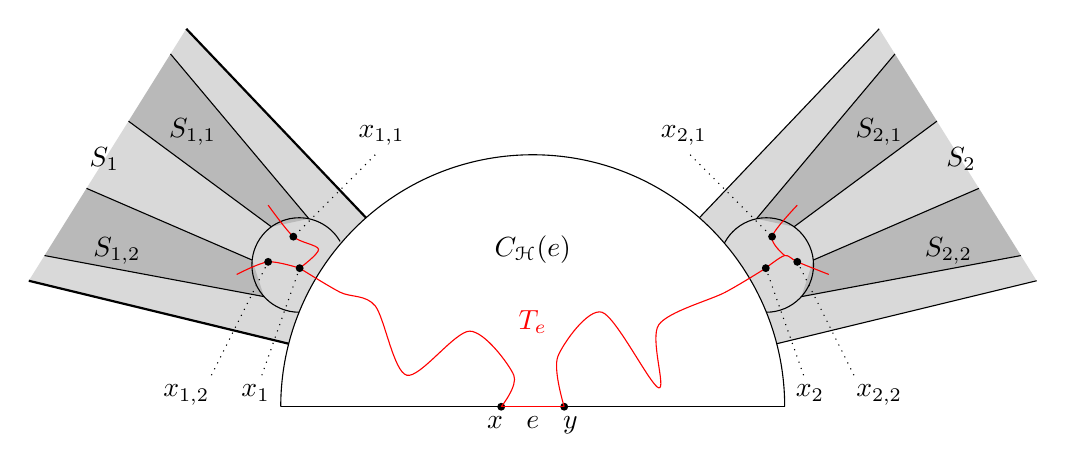
\begin{tikzpicture}[thick, scale=0.8]
        %Side S1, cell C_1, plus shading
        \draw [name path = S1A] (-3.87298,1) to (-8,2);
        \draw [name path = S1B](-2.64575,3) to (-5.5,6);
        \tikzfillbetween[of=S1B and S1A] {opacity=.15}
    
        \draw [name path = S11A] (-4.2654,1.7482) to (-7.75,2.4);
        \draw [name path = S11B] (-4.4539,2.3284) to (-7.0833,3.4667);
        \tikzfillbetween[of=S11B and S11A] {opacity=0.15}    
        \draw [name path = S12A] (-4.1488,2.8568) to (-6.4167,4.5333);
        \draw [name path = S12B] (-3.5521,2.9836) to (-5.7500,5.6000);
        \tikzfillbetween[of=S12B and S12A] {opacity=0.15} 
        \draw [name path = Arc2, black] (-3.708,1.5) arc (270:30:0.75);
        \draw (-6.8,3.6) node[above] {$S_1$};
        \draw (-5.4,4) node[above] {$S_{1,1}$};
        \draw (-6.6,2.1) node[above] {$S_{1,2}$};
    
        %Side S2, cell C_2, plus shading
        \draw [name path = S2A] (3.87298,1) to (8,2);
        \draw [name path = S2B](2.64575,3) to (5.5,6);
        \tikzfillbetween[of=S2B and S2A] {opacity=.15}
        \draw [name path = S21A] (4.2654,1.7482) to (7.75,2.4);
        \draw [name path = S21B] (4.4539,2.3284) to (7.0833,3.4667);
        \tikzfillbetween[of=S21B and S21A] {opacity=0.15}    
        \draw [name path = S22A] (4.1488,2.8568) to (6.4167,4.5333);
        \draw [name path = S22B] (3.5521,2.9836) to (5.7500,5.6000);
        \tikzfillbetween[of=S22B and S22A] {opacity=0.15} 
        \draw [name path = Arc3, black] (3.708,1.5) arc (270:-90:0.75);
        \draw (6.8,3.6) node[above] {$S_2$};
        \draw (5.5,4) node[above] {$S_{2,1}$};
        \draw (6.6,2.1) node[above] {$S_{2,2}$};
    
        %Ball B1 and stuff inside of it
        \draw [name path = Arc, fill=white](-4,0) arc (180:0:4);
        \node[big dot] (x) at (-0.5,0) {};
        \draw (-0.6,0) node[below] {$x$};
        \node[big dot] (y) at (0.5,0) {};
        \draw (0.6,0) node[below] {$y$};
        \draw (0,0) node[below] {$e$};
        \draw (-4,0) to (4,0);
        \draw[red] (-0.5,0) to (0.5,0);
        \node at (0,2.5) {$C_{\cH}(e)$};
        \draw [name path = T1, red] plot [smooth]  coordinates {(-0.5,0) (-0.3,0.5)  (-1,1.2) (-2,0.5) (-2.5,1.6) (-3.0554, 1.8167)(-3.7,2.2)};
        \draw [name path = T2, red] plot [smooth]  coordinates {(0.5,0) (0.4,0.8)  (1.1,1.5) (2,0.3) (2,1.3) (3.0554, 1.8167) (3.7,2.2)};

        \draw (0,1) node[above,red] {$T_e$};

        %red tree inside of C1
        \draw [name path = T11, red] plot [smooth]  coordinates {(-3.7,2.2) (-4.2,2.3) (-4.7,2.1)};
        \draw [name path = T12, red] plot [smooth]  coordinates {(-3.7,2.2) (-3.4,2.5) (-3.8,2.7) (-4.2,3.2)};
        \node[big dot] (x1) at (-3.7,2.2) {};
        \draw (-4.4,0.5) node[below] {$x_1$};
        \node[big dot] (x11) at (-4.2,2.3) {};
        \node[big dot] (x12) at (-3.8,2.7) {};
        \draw[dotted] (-4.3,0.5) to (x1);
        \draw[dotted] (-5.1,0.5) to (x11);
        \draw (-5.5,0.5) node[below] {$x_{1,2}$};
        \draw[dotted] (-2.5,4) to (x12);
        \draw (-2.4,4) node[above] {$x_{1,1}$};
    
        %red tree inside of C2
    
        \draw [name path = T22, red] plot [smooth]  coordinates {(3.7,2.2) (4,2.4) (4.2,2.3) (4.7,2.1)};
        \draw [name path = T21, red] plot [smooth]  coordinates {(4,2.4) (3.8,2.7) (4.2,3.2)};
        \node[big dot] (x21) at (4.2,2.3) {};
        \node[big dot] (x22) at (3.8,2.7) {};
        \node[big dot] (x2) at (3.7,2.2) {};
        \draw[dotted] (4.3,0.5) to (x2);
        \draw (4.4,0.5) node[below] {$x_2$};
        \draw[dotted] (5.1,0.5) to (x21);
        \draw (5.5,0.5) node[below] {$x_{2,2}$};
        \draw[dotted] (2.5,4) to (x22);
        \draw (2.4,4) node[above] {$x_{2,1}$};
        \end{tikzpicture}	
    \end{center}
    \caption{Illustration to the proof of Lemma~\ref{lem:trees_on_edges}. The red tree depicts the desired $T_e$.}\label{fig:Te}
    \end{figure}

\end{proof} 

\end{document}
